\documentclass[11pt]{article}
\usepackage{fullpage}
\usepackage{amsmath}    % need for subequations
%\usepackage{graphicx}   % need for figures
\usepackage{verbatim}   % useful for program listings
\usepackage{color}      % use if color is used in text
\usepackage{subfigure}  % use for side-by-side figures
\usepackage{hyperref}   % use for hypertext links, including those to external documents and URLs
\usepackage[pdftex]{graphicx}
\usepackage{sidecap}
\usepackage{wrapfig}


\title{CMSC 12300 Final Project}
\author{Andy Liu and Nelson Auner}
\begin{document}
\maketitle
\section{Introduction}

Our project investigates the use of census data to  predict whether a household self-reports that its income is over or under \$50,00. Our goals, put succintly, were to

\begin{enumerate}
  \item find and use a relevant prediction algorithm 
  \item test relevant models and select the best one, and
  \item develop an accurate estimation of our model's prediction of a similar, yet different data set.
\end{enumerate}
 

To do so, we used R and Python, deployed on personal computers as well as AWS, to implement logistical regression of various combinations of regressors. We took the best models, as defined by their performance within the training set, and subjected them to cross-validation. To deal with missing data, we utilized k nearest neighbors to "fill in" missing variables with the nearest closest observation.

 Our results suggest the following: Education as a stand-alone predictor is a very good model, with around 5.4\% false positive rate and .5\% false negative rate. By very good, however, we mean compared to other non-trivial (majority classifier) models, considering that the relative lack of diversity in our responses, given an absolute error weighting, favors a classification scheme with all-negative predictions. 


\section{Description of the Data set}
Our analysis is on the Census-Income (KDD) Data Set, a classic machine learning dataset of census data from the 1994 and 1995 Current Population Surveys conducted by the U.S. Census Bureau.

%It is also an interesting dataset for business/marketing purposes, given that predicting a household's income from semi-observeable characteristics is useful for understanding consumers for a possible product. 

The actual data is made freely available from 
\href{http://archive.ics.uci.edu/ml/datasets/Census-Income+%28KDD%29}{the UC-Irvine Machine Learning Repository}, and consists of 46 variables (see the appendix for a full list), with features such as race, capital gains, country of birth of parents, and weeks worked in the year. Because the census data if completed by participants on a voluntary basis, many variables had more missing observations than observed observations.  This is a challenging statistical problem because a household's decision to respond or not to a given question may be correlated with their household income, our choice variable of prediction, normal regression methods will result in inconsistent estimators. For example, for a standard regression model $Y = X\beta$, we would have: 
\begin{equation}
E(y_i|x_i) = x_i \beta + E(y_i | x_j = NA)
\end{equation}
where $x_j$ represents the variables $j = \{j_1, j_2,...,j_k\}$ with $x_j$ not reported. Put intuitively, the second term $E(y_i | x_j = NA)$ descibes how we would alter our prediction given that we have $NA$ in columns $j$; for example, it is possible that wealthier households are more likely to not self-report capital gains.$($Another problem all-together is that households could have purposefully mis-reported-a complexity that we avoid all-together to simplify our analysis$)$. The KNN method (described later) seeks to alleviate, but does not solve this problem. Perhaps due to this interaction between household income and missing data, several variables that intuitively would be a very good measure of household income, like wage/hr, weeks worked per year, and capital gains, are not only missing in many observations, but are not good predictors of household income. 

One of the most pertinant characteristic of the data set is that the "over 50K" variable only takes on a value of true for 6.2% of the observations. As we noted in our original proposal, this means that a majority classifiers--predicting that income is under 50K for all observations, would have been "93.8% accurate". However, this is not a useful predictor, since we do not know if a set of new observations would be reprentative at all of our current data. In addition, it's important to consider weighting the relative importance of assigning a false positive vs. a false negative: for a business/marketing application of the data, it may be more important to predict all of the observations with income > \$50K, than correctly predict observation under \$50K. In this sense, the majority classifier is undesireable, asit predicts no observations with income > \$50K, regardless of information.

\section{ Logistic Regression}
The task of predicting whether a household self reports that its income is over or under \$50,000 is a binary classification, as our outcome takes a value of either true $($income over \$50K$)$ or false $($income under \$50K $)$.  We decided early on in the project to use logistic regression, and aim to find the best classification method within the subset of logistic regression classifiers. Logistic regression transforms the predictors to
\begin{equation}
\pi(X) = \frac{e^{(X\beta)}}{1+e^{(X\beta)}}
\end{equation}

which looks like:
\begin{figure}[h!]
\centering
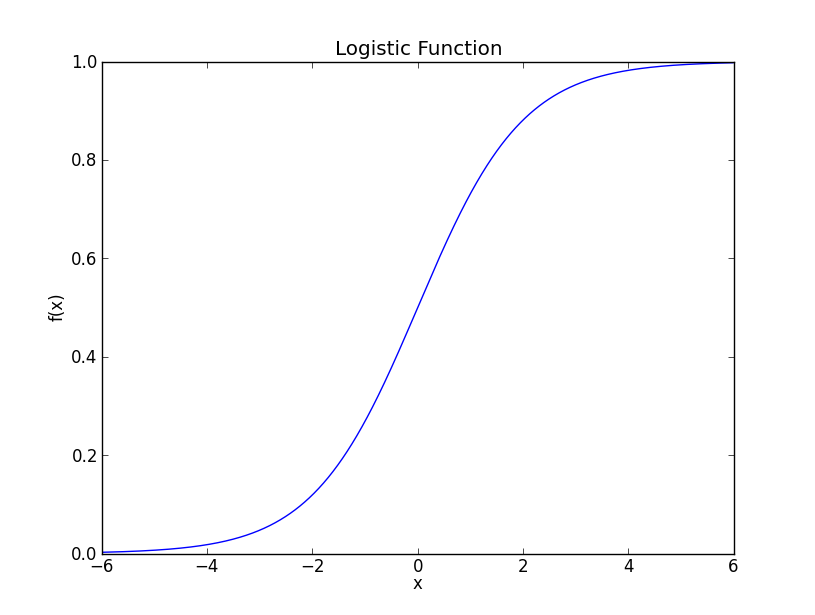
\includegraphics[width = 7cm]{logisticfunction.png}
\caption{A graph of the logistic function for reference, graphed by the authors using the numpy module of python}
\end{figure}


This function can be viewed as a CDF $($cumulative density function$)$ and closely mirrors that of a normal distribution, and projects the space of $X \beta$ to the interval $[0,1]$, allowing us to view the result as the probability that our outcome is 1. Our reasons for selecting a logistic regression model are simple: although it is more complicated than a basic regression mode $Y = X\beta$, logistic regression allows us to predict a binary outcome, while resulting in more interpretable coefficients $\beta$ than "black box" methods such as neural networks or random forest. 

\section{Initial analysis}
Our inital analysis was done in R, and much work was required to find and adapt the necessary statistical methods for use in python. 
We used the Akaike Information Criteria (AIC), defined as $AIC = 2k - 2ln(L)$, where $k$ is the number of the parameters in the model, and $L$ is the maximized value of the likelihood function - in our case, the logistical regression equation defined above. By maximizing AIC, we produced a subset of predictors that AIC evaluated as the "best" predictor sets. We noticed that among single-variable predictive methods, the education variable was one of the most effective, with a false positive error rate of 5% false negative error rate of .7%. However, these rates are not accurate measures of performance, because we are testing our predictor with the same data we used to train. 

\section{Filling in missing observations with KNN}
Andy spits his magic here. 

\section{Cross Validation}
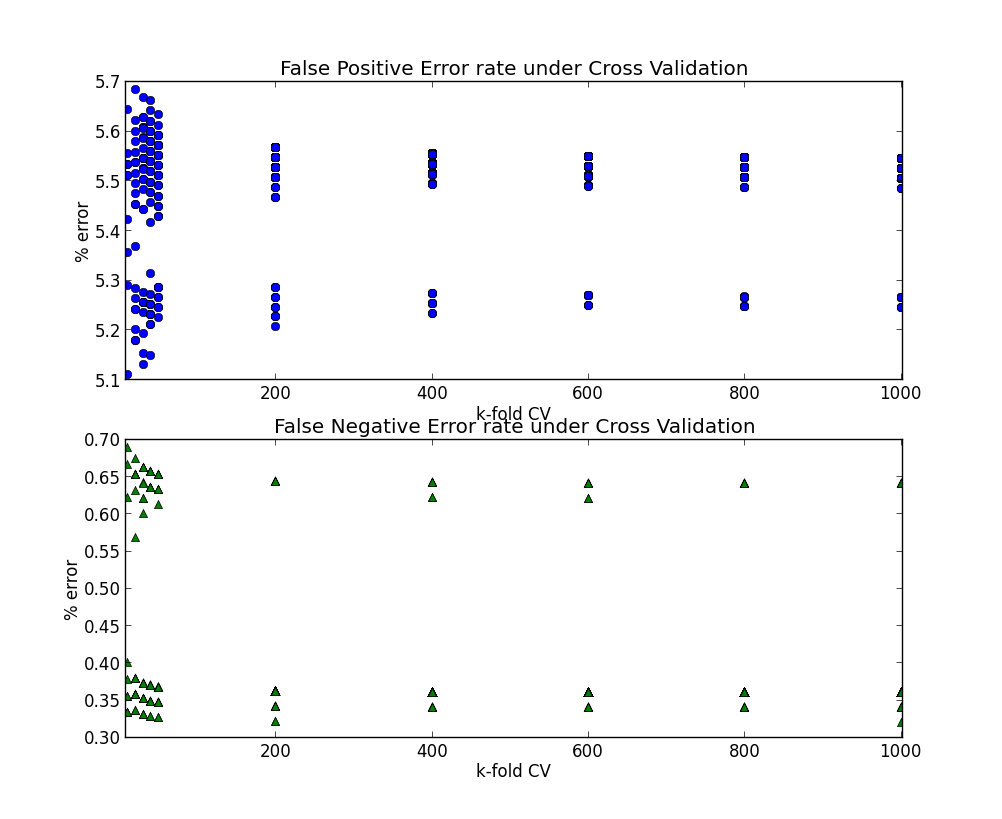
\includegraphics[width = 20cm]{CV_5K_1Kfold.png}
\end{document}


\section{appendix}
age	 AAGE 
class of worker	 ACLSWKR 
industry code	 ADTIND 
occupation code	 ADTOCC 
adjusted gross income	 AGI 
education	 AHGA 
wage per hour	 AHRSPAY 
enrolled in edu inst last wk	 AHSCOL 
marital status	 AMARITL 
major industry code	 AMJIND 
major occupation code	 AMJOCC 
mace	 ARACE 
hispanic Origin	 AREORGN 
sex	 ASEX 
member of a labor union	 AUNMEM 
reason for unemployment	 AUNTYPE 
full or part time employment stat	 AWKSTAT 
capital gains	 CAPGAIN 
capital losses	 CAPLOSS 
divdends from stocks	 DIVVAL 
federal income tax liability	 FEDTAX 
tax filer status	 FILESTAT 
region of previous residence	 GRINREG 
state of previous residence	 GRINST 
detailed household and family stat	 HHDFMX 
detailed household summary in household	 HHDREL 
instance weight	 MARSUPWT 
migration code-change in msa	 MIGMTR1 
migration code-change in reg	 MIGMTR3 
migration code-move within reg	 MIGMTR4 
live in this house 1 year ago	 MIGSAME 
migration prev res in sunbelt	 MIGSUN 
num persons worked for employer	 NOEMP 
family members under 18	 PARENT 
total person earnings	 PEARNVAL 
country of birth father	 PEFNTVTY 
country of birth mother	 PEMNTVTY 
country of birth self	 PENATVTY 
citizenship	 PRCITSHP 
total person income	 PTOTVAL 
own business or self employed	 SEOTR 
taxable income amount	 TAXINC 
fill inc questionnaire for veteran's admin	VETQVA 
veterans benefits	 VETYN 
weeks worked in year	 WKSWORK 